\documentclass[professionalfonts,compress,unicode]{beamer}

\usepackage{amsmath,amssymb}
\usepackage{empheq}
\usepackage[utf8]{inputenc}

\usepackage[russian]{babel}

\usepackage{ifthen}

\def\[#1\]{\begin{align*}#1\end{align*}}

\newcommand\myframe[3][dup]{
\ifthenelse{\equal{#1}{}}{}{\ifthenelse{\equal{#1}{dup}}{\subsection{#2}}{\subsection{#1}}}
\frame{\frametitle{#2}{#3}}%
}

\usetheme{Warsaw}
\usecolortheme{uranix}

\setbeamertemplate{headline}
{%
  \begin{beamercolorbox}[sep=0.3cm,wd=\paperwidth]{section in head/foot}%
    \usebeamerfont{frametitle}%
    \vbox{}\vskip-1ex%
    \strut\insertsectionhead\strut\par%
    \vskip-1ex%
  \end{beamercolorbox}%
}
\setbeamertemplate{navigation symbols}{}
\setbeamertemplate{footline}{}
\setbeamertemplate{caption}[numbered]

\renewcommand{\thefootnote}{\fnsymbol{footnote}}

\graphicspath{{images//}}

\title[Уравнение теплопроводности]{Уравнения параболического типа\\Уравнение теплопроводности}
\author[Цыбулин И.В.]{Скалько Юрий Иванович\\
\textbf{Цыбулин Иван}}
\date{}
%\vspace{0.3cm}

\newcommand{\cutefrac}[2]{{}^{#1}\!/{\!}_#2}
\newcommand{\half}{\cutefrac{1}{2}}

\begin{document}

{
\setbeamertemplate{headline}[default]
\frame{\titlepage}
}

\section{Одномерное уравнение теплопроводности}

\myframe{Уравнение теплопроводности}
{
	Типичный представитель уравнений параболического типа --- уравнение теплопроводности
	\[
	\frac{\partial u}{\partial t} = \frac{\partial}{\partial x}\left(\varkappa \frac{\partial u}{\partial x}\right).
	\]
	Будем также рассматривать случай $\varkappa = \operatorname{const}$
	\[
	\frac{\partial u}{\partial t} = \varkappa \frac{\partial^2 u}{\partial x^2}
	\]
	Уравнение описывает распространение тепла, диффузию вещества, вязкие процессы и т.п.
}

\myframe{Простейшая схема}
{
	Запишем простейшую явную схему для уравнения теплопроводности
	\[
	\frac{u^{n+1}_m - u^n_m}{\tau} = \frac{\varkappa_{m+\half}\frac{u^n_{m+1}-u^n_m}{h}-\varkappa_{m-\half}\frac{u^n_m-u^n_{m-1}}{h}}{h}
	\]
	Похожая аппроксимация встречалась в задаче Штурма-Лиувилля (там она обеспечивала диагональное преобладание в системе уравнений).
	
	В точке $(t_n,x_m)$ правая часть аппроксимирована с порядком $O(h^2)$, а левая с порядком $O(\tau)$. Значит порядок аппроксимации схемы не 
	хуже $O(\tau+h^2)$.
}

\myframe{Простейшая схема. Аппроксимация}
{
	Запишем разложения точного решения и коэффициента теплопроводности в ряд Тейлора в окрестности $(t_n,x_m)$ 
	\[
		[u]^{n+1}_m &= [u]^n_m + \tau [u_t]^n_m + \frac{\tau^2}{2} [u_{tt}]^n_m + O(\tau^3)\\
		[u]^n_{m\pm 1} &= [u]^n_m \pm h [u_x]^n_m + \frac{h^2}{2} [u_{xx}]^n_m \pm \frac{h^3}{6} [u_{xxx}]^n_m + \frac{h^4}{24} [u_{xxxx}]^n_m + O(h^5)\\
		[\varkappa]^n_{m\pm \half} &= [\varkappa]^n_m \pm \frac{h}{2} [\varkappa_x]^n_m + \frac{h^2}{8} [\varkappa_{xx}]^n_m \pm \frac{h^3}{48} [\varkappa_{xxx}]^n_m + O(h^4)
	\]
	Подставляя эти разложения в разностную схему и собирая слагаемые при одинаковых степенях $h$, получаем
	\[
	&\varkappa_{m+\half}\left(u^n_{m+1}-u^n_m\right)-\varkappa_{m-\half}\left(u^n_m-u^n_{m-1}\right) = \\
	&\Big([\varkappa_x]^n_m[u_x]^n_m + [\varkappa]^n_m[u_{xx}]^n_m\Big)h^2 + O(h^5) +\\ 
	&\Big([\varkappa_{xxx}]^n_m[u_x]^n_m + 3[\varkappa_{xx}]^n_m[u_{xx}]^n_m + 4[\varkappa_x]^n_m[u_{xxx}]^n_m + 2[\varkappa]^n_m[u_{xxxx}]^n_m\Big) h^4
	\]
}

\myframe[]{Простейшая схема. Аппроксимация}
{
	Заметим, что $\varkappa_xu_x + \varkappa u_{xx} \equiv (\varkappa u_x)_x$
	\[
	\delta &= \frac{\tau}{2}[u_{tt}]_m^n - \\
	&\Big([\varkappa_{xxx}]^n_m[u_x]^n_m + 3[\varkappa_{xx}]^n_m[u_{xx}]^n_m + 4[\varkappa_x]^n_m[u_{xxx}]^n_m + 2[\varkappa]^n_m[u_{xxxx}]^n_m\Big) h^2 =\\
	&=O(\tau+h^2)
	\]
}

%\myframe{Область зависимости}
%{
%	Область зависимости численного решения по данной явной четырехточечной схеме --- конус с наклоном образующих $\tau / h$.
%	
%	А вот область зависимости точного решения сложнее. Формально, решение уравнения теплопроводности зависит от значения в \emph{любой}
%	точке. В бесконечном пространстве верна формула Пуассона
%	\[
%	u(t,x) = \int_{-\infty}^{\infty} \frac{u(0, \xi)}{\sqrt{4 \varkappa \pi t}} e^{-\frac{(x-\xi)^2}{4\varkappa t}} d\xi.
%	\]
%	Видно, что \emph{существенно} решение зависит при $(x-\xi)^2 \lesssim 2 \varkappa t$, то есть областью зависимости можно назвать параболу 
%	$(x-\xi)^2 = 2 \varkappa t$
%}
%
%\myframe[]{Область зависимости}
%{
%	\begin{figure}%
%	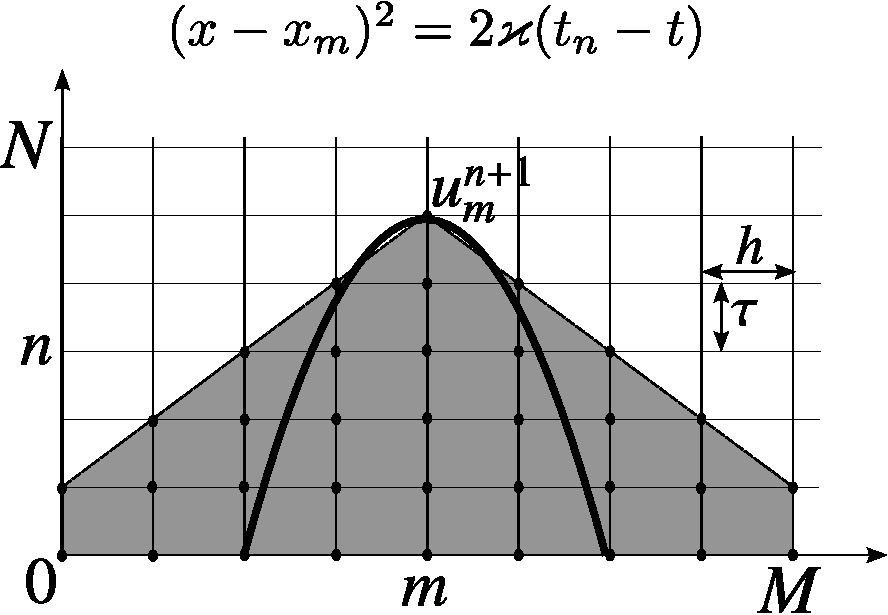
\includegraphics[width=0.5\columnwidth]{grid_dep2.pdf}%
%	\end{figure}
%	
%	Чтобы задача была устойчива, все узлы, попавшие в область зависимости дифференциальной задачи попали и в область зависимости
%	разностной задачи. То есть необходимое условие устойчивости явной схемы уже выглядит как $\frac{\tau}{h^2} < O(1)$
%}

\myframe{Устойчивость явной схемы}
{
	Если схема монотонна, то доказательство устойчивости проводится в полной аналогии с доказательством устойчивости монотонных схем 
	для уравнения переноса. Найдем условие монотонности схемы, для этого перепишем ее в разрешенной форме
	\[
	u^{n+1}_m &= u^n_m + \frac{\tau}{h}\left(\varkappa_{m+\half}\frac{u^n_{m+1}-u^n_m}{h}-\varkappa_{m-\half}\frac{u^n_m-u^n_{m-1}}{h}\right)\\
	u^{n+1}_m &= \left(1 - \frac{\tau(\varkappa_{m+\half}+\varkappa_{m-\half})}{h^2}\right)u^n_m 
	+\frac{\tau}{h^2}\varkappa_{m-\half}u^n_{m-1} 
	+\frac{\tau}{h^2}\varkappa_{m+\half}u^n_{m+1}
	\]
	Условие устойчивости
	\[
	\frac{\left(\varkappa_{m+\half}+\varkappa_{m-\half}\right)\tau}{h^2} < 1
	\]
	справедливо при
	\[
	\frac{2\tau\max\varkappa}{h^2} < 1
	\]
}

\myframe{Устойчивость по спектральному признаку}
{
	Условие монотонности не всегда является необходимым, проверим достаточность по спектральному признаку. Для этого нужно избавится от граничных условий,
	превратив начально-краевую задачу в задачу Коши, обнулить правую часть и рассмотреть возмущение специального вида $e^{i \alpha m}$. 
	Необходимо также <<заморозить>> коэффициент $\varkappa$, то есть сделать его константой $\varkappa = \operatorname{const}$.
	
	Будем искать решение в виде $u^n_m = \lambda^n e^{i \alpha m}$
	
	\[
	\frac{\lambda - 1}{\tau} &= \varkappa\frac{e^{-i \alpha} -2 + e^{i\alpha}}{h^2} = -\frac{4\varkappa}{h^2} \sin^2 \frac{\alpha}{2}\\
	\lambda &= 1 - \frac{4\varkappa\tau}{h^2}\sin^2 \frac{\alpha}{2}\\
	|\lambda| &< 1 \Rightarrow \frac{2\varkappa\tau}{h^2} < 1
	\]
}

\myframe{Выводы для явной схемы}
{
	Итак, при исследовании как спектральным признаком, так и по определению получается условие устойчивости 
	\[
	\frac{\varkappa\tau}{h^2} < \frac{1}{2}.
	\]
	На практике, такое ограничение является довольно неприятным, и его стараются ослабить.
}

\myframe{Неявная схема}
{
	Построим схему по аналогии с простейшей явной, только аппроксимируем производную по пространству на верхнем слое по времени.
	\[
	\frac{u^{n+1}_m - u^n_m}{\tau} = \frac{\varkappa_{m+\half}\frac{u^{n+1}_{m+1}-u^{n+1}_m}{h}-\varkappa_{m-\half}\frac{u^{n+1}_m-u^{n+1}_{m-1}}{h}}{h}
	\]
	Аналогично явной схеме, ее порядок аппроксимации $O(\tau+h^2)$.
	
	Исследовать такую схему по определению на устойчивость уже практически невозможно. Заморозим коэффициент $\varkappa = \operatorname{const}$
	и применим спектральный признак
}

\myframe{Спектральный признак. Неявная схема}
{
	\[
	\frac{\lambda - 1}{\tau} &= \lambda\varkappa\frac{e^{-i \alpha} -2 + e^{i\alpha}}{h^2} = -\lambda\frac{4\varkappa}{h^2} \sin^2 \frac{\alpha}{2}\\
	\lambda &= 1 - \lambda\frac{4\varkappa\tau}{h^2}\sin^2 \frac{\alpha}{2}\\
	\lambda &= \frac{1}{1 + \frac{4\varkappa\tau}{h^2}\sin^2 \frac{\alpha}{2}}\\
	\]
	Теперь $\lambda$ меньше единицы по модулю всегда при любых соотношениях между $\tau$ и $h$, то есть схема безусловно устойчива.
}

\myframe{Неявная схема}
{
	Но платой за безусловную устойчивость оказалась неявность схемы. Теперь на каждом шаге по времени необходимо решать систему уравнений для определения $u^{n+1}$.
	\[
	\left(1+\tau\frac{\varkappa_{m+\half}+\varkappa_{m-\half}}{h^2}\right)u^{n+1}_m 
	-\frac{\tau\varkappa_{m+\half}}{h^2}u^{n+1}_{m+1} 
	-\frac{\tau\varkappa_{m-\half}}{h^2}u^{n+1}_{m-1}
	= u^n_m
	\]
	
	Вместе с граничными условиями
	\[
	u^{n+1}_0 = \alpha^{n+1}\\
	u^{n+1}_M = \beta^{n+1}
	\]
	
	мы получаем трехдиагональную систему. Более того, в этой системе имеется диагональное преобладание, значит алгоритм прогонки в этом случае гарантировано будет устойчив.
	Таким образом, решение по неявной схеме всего в несколько раз медленнее решения по явной схеме.
}

\section{Многомерное уравнение теплопроводности}

\myframe{Двумерное уравнение теплопроводности}
{
	Рассмотрим двумерное уравнение теплопроводности с постоянным коэффициентом $\varkappa = \operatorname{const}$
	\[
	\frac{\partial u}{\partial t} = \varkappa \left(\frac{\partial^2 u}{\partial x^2} + \frac{\partial^2 u}{\partial y^2}\right)
	\]
}

\myframe{Простейшие аппроксимации}
{
	У сеточной функции теперь 3 индекса $(m,n)$ --- пространственные индексы по $x$ и $y$, $p$ --- временной индекс.
	
	Условимся операторами $\Lambda_{xx}, \Lambda_{yy}$ обозначать разностные вторые производные, то есть
	\[
	\Lambda_{xx} u^p_{n,m} = \frac{u^p_{m+1,n} - 2 u^p_{m,n} + u^p_{m-1,n}}{h^2}\\
	\Lambda_{yy} u^p_{n,m} = \frac{u^p_{m,n+1} - 2 u^p_{m,n} + u^p_{m,n-1}}{h^2}
	\]
	
	Простейшая явная схема записывается в этих обозначениях как
	\[
	&\frac{u^{p+1}_{m,n} - u^p_{m,n}}{\tau} = \varkappa \left(\Lambda_{xx} u^p_{m,n} + \Lambda_{yy} u^p_{m,n} \right)\\
	&u^0_{m,n} = \varphi_{m,n}\\
	&\left. u^p_{m,n} \right|_{\Gamma} = \psi^p_{m,n}|_{(x,y) \in \Gamma}\\
	\]
}

\myframe{Свойства операторов вторых производных}
{
	Важной особенностью операторов $\Lambda_{xx}$ и $\Lambda_{yy}$ является то, что они, как и операторы $\frac{\partial^2}{\partial x^2}, \frac{\partial^2}{\partial y^2}$ коммутируют
	\[
	\Lambda_{xx}\Lambda_{yy} u_{m,n} = \Lambda_{yy}\Lambda_{xx} u_{m,n}
	\]
	
	Также, для этих операторов известны собственные числа и собственные вектора
	\[
	\Lambda_{xx} e^{i \alpha m} = -\frac{4}{h^2} \sin^2 \frac{\alpha}{2} e^{i \alpha m}
	\]
	сравните с 
	\[
	\frac{\partial^2}{\partial x^2} e^{\frac{i \alpha x}{h}} = -\frac{\alpha^2}{h^2} e^{\frac{i \alpha x}{h}}
	\]
}

\myframe{Аппроксимация}
{
	Операторы $\Lambda_{xx}, \Lambda_{yy}$ аппроксимируют вторые производные со вторым порядком
	\[
	\Lambda_{xx} [u]^p_{m,n} = [u_{xx}]^p_{m,n} + \frac{h^2}{12}[u_{xxxx}]^p_{m,n} + O(h^4),
	\]
	воспользуемся этим для нахождения ошибки аппроксимации
	\[
	&\frac{[u]^{p+1}_{m,n} - [u]^p_{m,n}}{\tau} = \varkappa \left(\Lambda_{xx} [u]^p_{m,n}+\Lambda_{yy} [u]^p_{m,n}\right) + \delta\\
	&\delta = \frac{\tau}{2} [u_{tt}] + O(\tau^2) + \varkappa\frac{h^2}{12}([u_{xxxx}]^p_{m,n}+[u_{yyyy}]^p_{m,n}) + O(h^4) = O(\tau + h^2)
	\]
}
\myframe{Устойчивость}
{
	Проверим устойчивость по спектральному признаку. Ищем решение в виде
	$ u^p_{m,n} = \lambda^p e^{i\alpha m} e^{i \beta n}$
	\[
	&\frac{\lambda - 1}{\tau} = \varkappa \left(-\frac{4}{h^2}\sin^2\frac{\alpha}{2}-\frac{4}{h^2}\sin^2\frac{\beta}{2}\right)\\
	&\lambda = 1 - \frac{4\varkappa\tau}{h^2} \left(\sin^2\frac{\alpha}{2}+\sin^2\frac{\beta}{2}\right)\\
	&|\lambda| < 1 \Rightarrow \frac{\varkappa\tau}{h^2} < \frac{1}{4}
	\]
	Схема является условно устойчивой с вдвое более жестким условием, чем для одномерной схемы
}

\myframe{Неявная схема}
{
	Изучим устойчивость неявной схемы
	\[
	\frac{u^{p+1}_{m,n} - u^p_{m,n}}{\tau} = \varkappa \left(\Lambda_{xx} u^{p+1}_{m,n} + \Lambda_{yy} u^{p+1}_{m,n} \right)
	\]
	Также ищем решение в виде $u^p_{m,n} = \lambda^p e^{i\alpha m} e^{i \beta n}$
	\[
	&\frac{\lambda - 1}{\tau} = \varkappa \lambda\left(-\frac{4}{h^2}\sin^2\frac{\alpha}{2}-\frac{4}{h^2}\sin^2\frac{\beta}{2}\right)\\
	&\lambda = \frac{1}{1 + \frac{4\varkappa\tau}{h^2} \left(\sin^2\frac{\alpha}{2}+\sin^2\frac{\beta}{2}\right)}\\
	&|\lambda| < 1
	\]
	Схема безусловно устойчива, как и в одномерном случае.
}

\myframe{Схемы расщепления}
{
	В двумерном случае матрица системы уже не трехдиагональная. Аналогичных быстрых методов для такой системы не существует.
	Выходом из положения являются различные методы расщепления. Рассмотрим на примере следующей схемы
	\[
	\frac{w^{p+1/2}_{m,n} - u^p_{m,n}}{\tau/2} = \varkappa \left(\Lambda_{xx} w^{p+1/2}_{m,n} + \Lambda_{yy} u^{p}_{m,n} \right)\\
	\frac{u^{p+1}_{m,n} - w^{p+1/2}_{m,n}}{\tau/2} = \varkappa \left(\Lambda_{xx} w^{p+1/2}_{m,n} + \Lambda_{yy} u^{p+1}_{m,n} \right)
	\]
	Шаг по времени разбивается на два полушага. На первом полушаге аппроксимация производной по $x$ неявная, по $y$ явная, на следующем полушаге --- наоборот.
}

\myframe{Исключение промежуточного слоя}
{
	Запишем схему в операторном виде
	\[
	w^{p+1/2} - u^{p} &= \frac{\varkappa\tau}{2}\left(\Lambda_{xx} w^{p+1/2} + \Lambda_{yy} u^p\right)\\
	u^{p+1} - w^{p+1/2} &= \frac{\varkappa\tau}{2}\left(\Lambda_{xx} w^{p+1/2} + \Lambda_{yy} u^{p+1}\right)\\
	\left(E - \frac{\varkappa\tau}{2}\Lambda_{xx}\right) w^{p+1/2} &= \left(E + \frac{\varkappa\tau}{2}\Lambda_{yy}\right) u^p\\
	\left(E - \frac{\varkappa\tau}{2}\Lambda_{yy}\right) u^{p+1} &= \left(E + \frac{\varkappa\tau}{2}\Lambda_{xx}\right) w^{p+1/2}\\
	\]
	Чтобы найти $W^{p+1/2}$ достаточно сделать прогонку по координате $x$, затем прогонку по координате $y$, чтобы найти $u^{p+1}$.
	Исключим $w^{p+1/2}$
	{\small
	\[
	u^{p+1} = \left(E - \frac{\varkappa\tau}{2}\Lambda_{yy}\right)^{-1} \left(E + \frac{\varkappa\tau}{2}\Lambda_{xx}\right) 
	\left(E - \frac{\varkappa\tau}{2}\Lambda_{xx}\right)^{-1} \left(E + \frac{\varkappa\tau}{2}\Lambda_{yy}\right) u^p\\
	\]
	}
}

\myframe{Аппроксимация схемы расщепления}
{
	{\small
	\[
	u^{p+1} = \left(E - \frac{\varkappa\tau}{2}\Lambda_{yy}\right)^{-1} \left(E + \frac{\varkappa\tau}{2}\Lambda_{xx}\right) 
	\left(E - \frac{\varkappa\tau}{2}\Lambda_{xx}\right)^{-1} \left(E + \frac{\varkappa\tau}{2}\Lambda_{yy}\right) u^p\\
	\]
	}
	Раскладывая операторы в ряд
	\[
	\left(E - \frac{\varkappa\tau}{2}\Lambda_{xx}\right)^{-1} = E + \frac{\varkappa\tau}{2}\Lambda_{xx} + \frac{\varkappa^2\tau^2}{4}\Lambda^2_{xx} + O(\tau^3)
	\]
	и перемножая, получаем
	{\small
	\[
	u^{p+1} = \left(E + \varkappa\tau(\Lambda_{xx} + \Lambda_{yy}) + \frac{\varkappa^2\tau^2}{2}(\Lambda_{xx} + \Lambda_{yy})^2 + O(\tau^3)\right) u^p\\
	\frac{u^{p+1}-u^p}{\tau} = \left(\Lambda_{xx} + \Lambda_{yy}\right) u^p + \frac{\varkappa^2\tau}{2}(\Lambda_{xx} + \Lambda_{yy})^2 u^p + O(\tau^2)
	\]
	}
	Ошибка аппроксимации
	\[
	\delta = \frac{\tau}{2}[u_{tt}]^p - \frac{\varkappa^2\tau}{2}\left(\frac{\partial^2}{\partial x^2}+\frac{\partial^2}{\partial y^2}\right)^2 u^p + O(\tau^2 + h^2)
	\]
}

\myframe[]{Аппроксимация схемы расщепления}
{
	Ошибка аппроксимации
	\[
	\delta = \frac{\tau}{2}[u_{tt}]^p - \frac{\varkappa^2\tau}{2}\left(\frac{\partial^2}{\partial x^2}+\frac{\partial^2}{\partial y^2}\right)^2 u^p + O(\tau^2 + h^2)
	\]
	
	На первый взгляд ошибка аппроксимации $O(\tau + h^2)$, но внимательно посмотрев, можно заметить, что на решении
	\[
	u_{tt} = \varkappa^2 \left(\frac{\partial^2}{\partial x^2}+\frac{\partial^2}{\partial y^2}\right)^2 u
	\]
	и первые два члена ошибки взаимно уничтожаются и оибка аппроксимации равна
	\[
	\delta = O(\tau^2 + h^2)
	\]
}


\myframe{Устойчивость схемы расщепления}
{
	{\small
	\[
	u^{p+1} = \left(E - \frac{\varkappa\tau}{2}\Lambda_{yy}\right)^{-1} \left(E + \frac{\varkappa\tau}{2}\Lambda_{xx}\right) 
	\left(E - \frac{\varkappa\tau}{2}\Lambda_{xx}\right)^{-1} \left(E + \frac{\varkappa\tau}{2}\Lambda_{yy}\right) u^p\\
	\]
	}
	Воспользуемся спектральным признаком
	\[
	u^p = \lambda^p e^{i \alpha m} e^{i \beta n} 
	\]
	Заметим, что $u^p$ --- собственная функция операторов $\Lambda$. Это позволяет заменить все операторы на собственные значения
	\[
	&\lambda = \frac{1}{1+\frac{4\varkappa\tau}{2h^2}\sin^2 \frac{\beta}{2}} 
	\left(1-\frac{4\varkappa\tau}{2h^2}\sin^2 \frac{\alpha}{2}\right)
	\frac{1}{1+\frac{4\varkappa\tau}{2h^2}\sin^2 \frac{\alpha}{2}}
	\left(1-\frac{4\varkappa\tau}{2h^2}\sin^2 \frac{\beta}{2}\right)\\
	&|\lambda| = \left|\frac{1-\frac{4\varkappa\tau}{2h^2}\sin^2 \frac{\alpha}{2}}{1+\frac{4\varkappa\tau}{2h^2}\sin^2 \frac{\alpha}{2}}\right|
	\left|\frac{1-\frac{4\varkappa\tau}{2h^2}\sin^2 \frac{\beta}{2}}{1+\frac{4\varkappa\tau}{2h^2}\sin^2 \frac{\beta}{2}}\right| < 1
	\]
	Данная схема также безусловно устойчива, имеет порядок $O(\tau^2+h^2)$ и один шаг <<стоит>> две прогонки
}

%%%%%%%%%%%%%%%%%%%%%%%%%%%%%%%%%%%%%%%%%%%%%%%
%%%%%%%%%%%%%%%%%%%%%%%%%%%%%%%%%%%%%%%%%%%%%%%
%%%%%%%%%                            %%%%%%%%%%
%%%%%%%%%%%%%%%%%%%%%%%%%%%%%%%%%%%%%%%%%%%%%%%
%%%%%%%%%%%%%%%%%%%%%%%%%%%%%%%%%%%%%%%%%%%%%%%
{
\setbeamertemplate{headline}[default] 
\frame{
	\begin{center}
	{\Huge Спасибо за внимание!}
	\end{center}
	\bigskip
	\begin{center}
	{\color{blue}{tsybulin@crec.mipt.ru}}
	\end{center}
	}
}

\end{document}
